\section{Results: Escape Across the Three Representations}
\label{sec:hull-escape-results}
\subsection{Native Clots and Their Own Projections}
In the first frozen frame, a tracer fit at 89.3\% of sampled hull positions in native 3D but at only 46.3\% in the eight-slab projection (Fig.~\ref{fig:hull-escape}A). At 30~min the corresponding fractions were 88.8\% and 50.0\%. Among positions where the tracer fit, a path to the hull was verified for all sampled native positions and, on average, for 98.5--98.9\% in the projections across the three snapshot ages. The remaining projected positions had unresolved connectivity.

\begin{figure*}[!t]
\centering
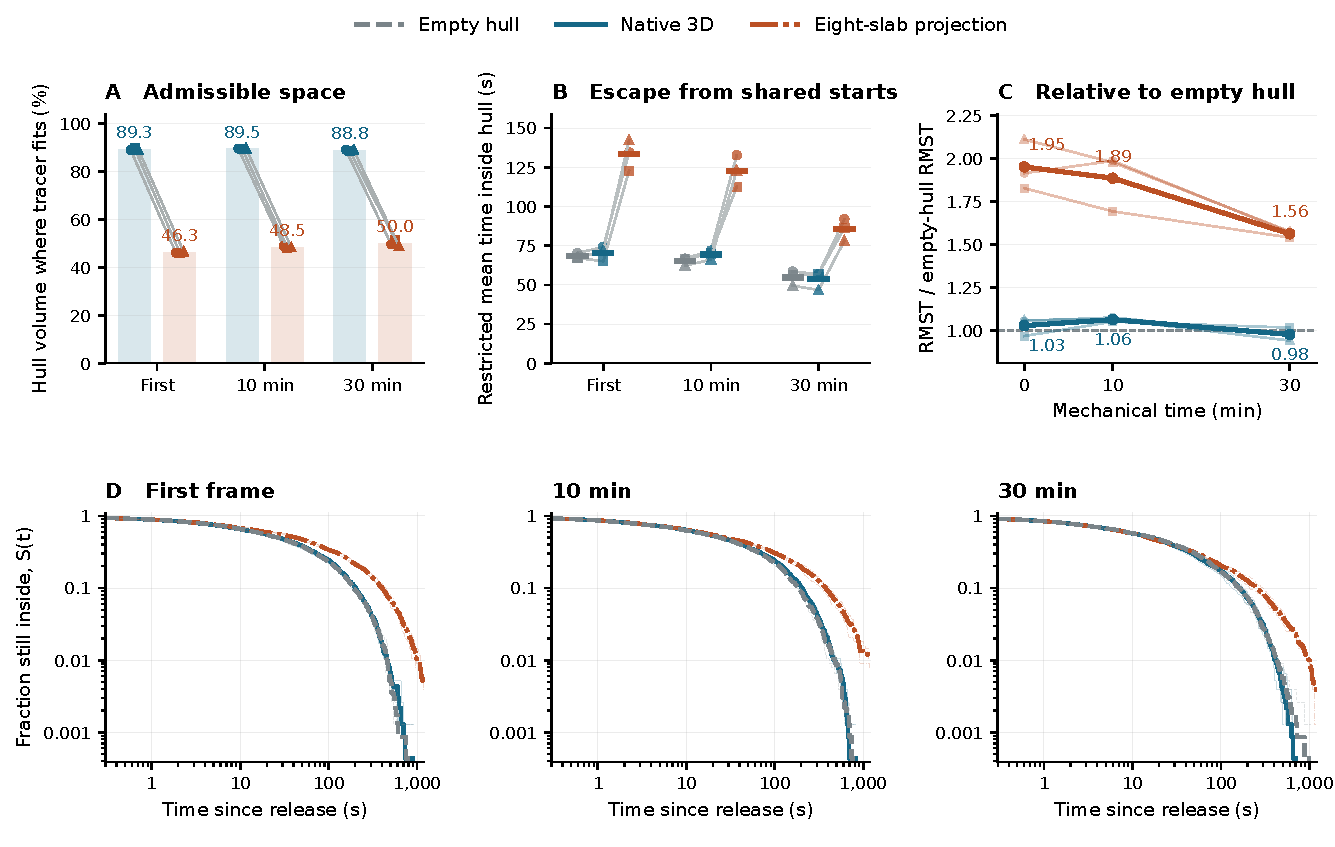
\includegraphics[width=\textwidth]{figures/hull_escape_paired.pdf}
\caption{Escape of a $0.5~\mu\mathrm m$ tracer in three paired clots. (A) Fraction of 8,192 uniformly sampled hull positions per clot and snapshot where the tracer fits. (B) Restricted mean time inside the hull (RMST through 1,200~s) for 768 shared starts per clot. Symbols distinguish clots; gray lines pair observations and horizontal ticks show means. (C) RMST divided by that clot's empty-hull RMST; bold lines average the three within-clot ratios. The first frame was saved at 0.01~s. (D) Survival since release on logarithmic axes; thin curves show individual clots and thick curves their means. At 1,200~s, 11, 25 and 9 of 2,304 projected tracers remained in the first, 10~min and 30~min snapshots, respectively; none remained in native 3D. Zero survival is not plotted.}
\label{fig:hull-escape}
\end{figure*}

Projection also delayed escape from the \emph{same} valid positions (Fig.~\ref{fig:hull-escape}B; Table~\ref{tab:hull-rmst}). Relative to each clot's matched empty hull, mean within-clot RMST ratios for the projection were 1.95, 1.89 and 1.56 in the first, 10~min and 30~min snapshots. Native ratios remained close to one (1.03, 1.06 and 0.98; Fig.~\ref{fig:hull-escape}C). The direct projection effect is the paired difference from native 3D, not the ratio to the empty hull. At 300~s of transport in the first snapshot, 14.8\% of tracers remained in the projection versus 4.5\% in native 3D (Fig.~\ref{fig:hull-escape}D). Trajectories still inside at the cutoff were censored, not classified as trapped.

\begin{table}[!htbp]
\centering\small
\caption{Restricted mean time inside the hull through 1,200~s (seconds). Each entry is a mean across three clots; $\Delta$ is projection minus native within clot.}
\label{tab:hull-rmst}
\setlength{\tabcolsep}{3.4pt}
\begin{tabular}{@{}lrrrr@{}}
\toprule
Snapshot & Empty & Native & Projected & $\Delta$ \\
\midrule
0.01~s & 68.3 & 70.2 & 133.2 & 63.0 \\
\specialrule{0.2pt}{1.5pt}{1.5pt}
10~min & 65.1 & 69.3 & 122.7 & 53.4 \\
\specialrule{0.2pt}{1.5pt}{1.5pt}
30~min & 54.7 & 53.5 & 85.4 & 31.9 \\
\bottomrule
\end{tabular}
\end{table}

The paired RMST increase ranged from 57.8 to 70.7~s across the three clots in the first frame, and from 29.3 to 35.0~s at 30~min. It was positive in all clots at all three base time steps. Halving the primary step changed individual RMST estimates by up to 12.8~s and survival by up to 2.5 percentage points at the four checkpoints (100, 300, 600 and 1,200~s). These checks support the direction of the effect, not numerical equivalence of the estimates.

\subsection{Projected Versus Independent Stacks}
At all three ages the independent stacks admitted a larger fraction of candidate centers than the projections, but a smaller fraction than native 3D (Fig.~\ref{fig:representation-bridge}A). In the independent stacks this fraction increased from 67.4\% to 76.8\% between the first and last states. At each age, a route to the hull was certified for more than 99.9\% of admissible starts on average. Of 4,608 released tracers per age, 3, 0 and 1 remained inside at 1,200~s in the primary runs at the first, 10 and 30~min states. Unresolved geometric connectivity and survival to the cutoff are distinct outcomes.

\begin{figure*}[!t]
\centering
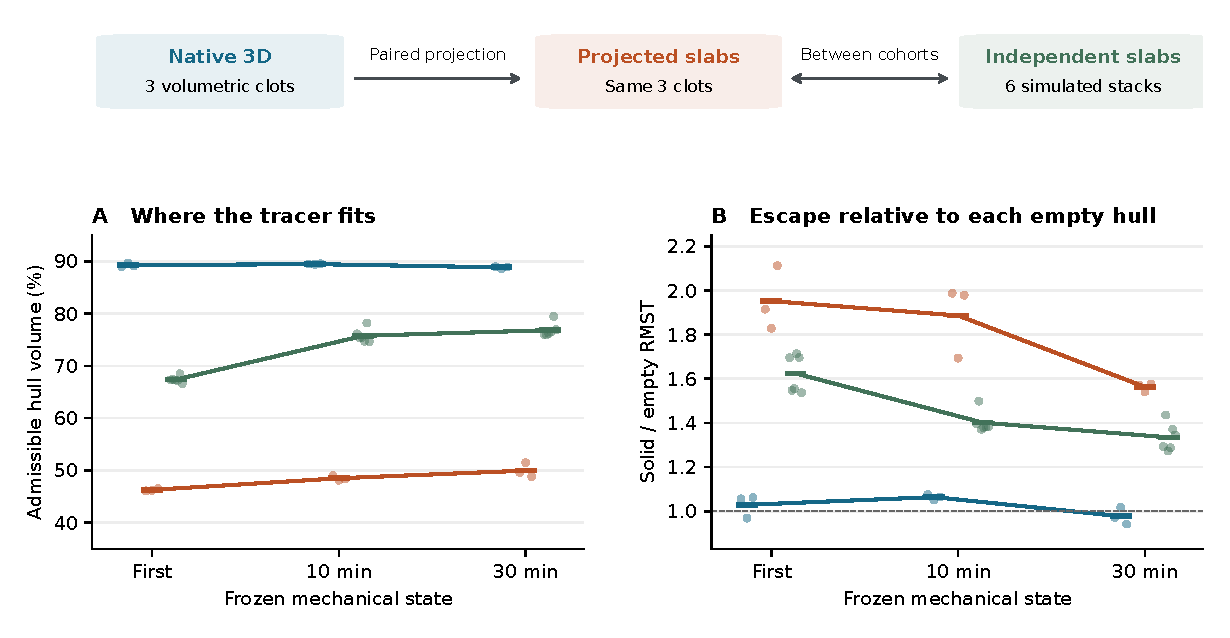
\includegraphics[width=0.94\textwidth]{figures/representation_bridge.pdf}
\caption{Two comparisons link three representations. The first arrow projects each simulated 3D clot; the second compares those projections with a separate cohort of independent stacks. (A) Percentage of the hull in which the tracer center fits. (B) Restricted mean time to escape divided by the empty-hull value for the same clot, age and release positions. The dashed line denotes no difference from the empty hull. Dots are clots; lines join cohort means across ages. Shared release positions apply within the native--projection pairs and within each independent stack--empty pair, not between cohorts.}
\label{fig:representation-bridge}
\end{figure*}

In the independent stacks, RMST decreased from $108.5\pm9.9$~s in the first frame to $87.4\pm3.7$~s at 10~min and $64.5\pm6.1$~s at 30~min (mean $\pm$ SD, six stacks). Their matched empty-hull means also decreased: 66.8, 62.4 and 48.3~s. The within-stack ratios were $1.62\pm0.09$, $1.40\pm0.05$ and $1.33\pm0.06$, respectively (Fig.~\ref{fig:representation-bridge}B). These mean ratios were below the projections and above native 3D at each age. For example, at 30~min the independent stacks and projections both retained tracers longer than their own empty hulls, whereas native 3D gave a ratio of 0.98. The between-cohort contrasts describe groups of clots; they are not paired projection effects.

Placing the independent hull at the outer slab faces rather than at the node midplanes increased its mean RMST to 129.4, 101.1 and 76.9~s. Its solid-to-empty ratios (1.70, 1.46 and 1.42) still fell between the native and projected means at all three ages. For the primary boundary, halving the base step changed individual solid RMSTs by at most 5.4~s and checkpoint survival by at most 2.0 percentage points. Every independent stack showed longer retention than its matched empty hull at all three tested steps. Absolute escape times remain sensitive to the chosen hull.
